\section{Auswertung}
\label{sec:Auswertung}


Die aus der auf dem Oszillator angezeigten Entladekurve entnommenen Messwerte werden in \ref{tab:tabelle1} dargestellt.

\begin{table}
  \centering
  \caption{Messwerte zur Entladekurve}
  \label{tab:tabelle1}
  \sisetup{table-format=1.1, per-mode=reciprocal}
  \begin{tblr}{
      colspec = {S[table-format=3.0] S[table-format=2.1] S},
      row{1} = {guard, mode=math},
    }
    \toprule
    t \mathbin{/} \unit{\second} \cdot 10^-3 [\pm 0.2]& U_c \mathbin{/} \unit{\volt} [\pm 0.4] & \\
    \midrule
    0   & 13.6 \\
    0.4 & 11   \\
    0.6 & 10   \\
    0.8 & 9.2  \\
    1.0 & 8.4  \\
    1.2 & 7.6  \\
    1.4 & 6.8  \\
    1.6 & 5.0  \\
    2.5 & 4.0  \\
    3.0 & 3.0  \\
    3.7 & 2.0  \\
    4.0 & 1.6  \\
    4.4 & 1.2  \\
    4.8 & 1.0  \\
    5.0 & 0.9  \\
    5.2 & 0.8  \\
    6.0 & 0.4  \\
    6.4 & 0    \\
    \bottomrule
  \end{tblr}
\end{table}

Nun wird in Abbildung \ref{fig:plot1} eine Fit-funktion mit polyfit \cite{numpy} erstellt, gefittet wird eine Funktion der gestalt:\\
\\
$\log{\frac{U_c}{U_0}} = a \cdot t + b$\\
\\
Die Parameter egeben sich zu:\\
$a = -561.333 ± 11.666$\\
$b = 1.389 ± 0.038$\\
\\
Um die Parameterberechung und das plotten zu ermöglichen wurde der letzte Messwert aus der Tabelle ignoriert.
\newpage

\begin{figure}
  \centering
  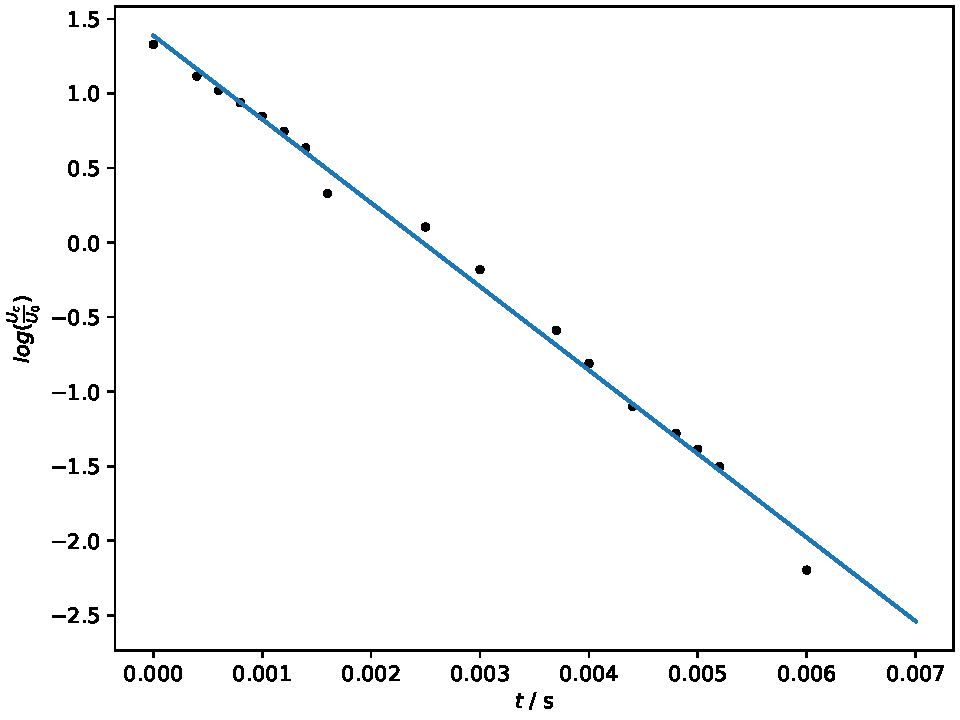
\includegraphics[width = 10cm]{plot1.pdf}
  \caption{Lineare Regression zur Bestimung der Zeitkonstante mithilfe der Entladungskurve}
  \label{fig:plot1}
\end{figure}

Da $a = -\frac{1}{RC}$, ist $RC = 0.00178\pm 0.00004$.



Eine weitere Methode die zeitkonstante RC zu bestimmen kann ausgeführt werden durch die Messung von der Amplitude unter variierender Frequenz der Wechselspannung.
Die Messwerte sind in Tabelle \ref{tab:tabelle2} aufgeführt.
\begin{table}
  \centering
  \caption{Messwerte zur Amplitude und Frequenz}
  \label{tab:tabelle2}
  \sisetup{table-format=1.1, per-mode=reciprocal}
  \begin{tblr}{
      colspec = {S[table-format=3.3] S[table-format=6.6] S},
      row{1} = {guard, mode=math},
      vline{2} = {2}{-}{text=\clap{$\pm$}},
    }
    \toprule
    \SetCell[c=2]{c} A \mathbin{/} \unit{\volt} & & F \mathbin{/} \unit{\hertz} [\pm 1] & \\
    \midrule
    6.8   & 0.4   &  50   \\
    4.8   & 0.4   &  100  \\
    1.2   & 0.4   &  500  \\
    0.6   & 0.2   &  1000 \\
    0.2   & 0.04  &  3000 \\
    0.12  & 0.04  &  5000 \\
    0.08  & 0.04  &  7000 \\
    0.06  & 0.02  &  10000\\
    0.05  & 0.02  &  12000\\
    0.04  & 0.01  &  15000\\
    0.035 & 0.01  &  17000\\
    0.034 & 0.004 &  19000\\
    0.032 & 0.004 &  20000\\
    0.03  & 0.002 &  22000\\
    \bottomrule
  \end{tblr}
\end{table}

\newpage

Anhand der Messwerte wird eine Ausgleichsfunktion der Gestalt:\\
\\
$U_c = \frac{1}{\sqrt(1+(F\cdot2\pi)\cdot a^2)}$ siehe \ref{eqn:amplitude2}\\
\\
mit curve-fit \cite{scipy} erstellt. $U_c$ ist dabei die Realtivamplitude $A/U_0$\\
\\
Die Parameter ergeben sich zu:\\
\\
$a = 0.00155 \pm 0.00007$\\
\\
Mit \ref{eqn:amplitude2} gilt also $RC = 0.00155 \pm 0.00007 $\\

Zum Zweck des Vergleichens wurde dieselbe Funktion noch einmal mit $RC = 0.00178$ geplottet. Der Graph ist zu sehen in Abbildung \ref{fig:plot2}.

\begin{figure}
  \centering
  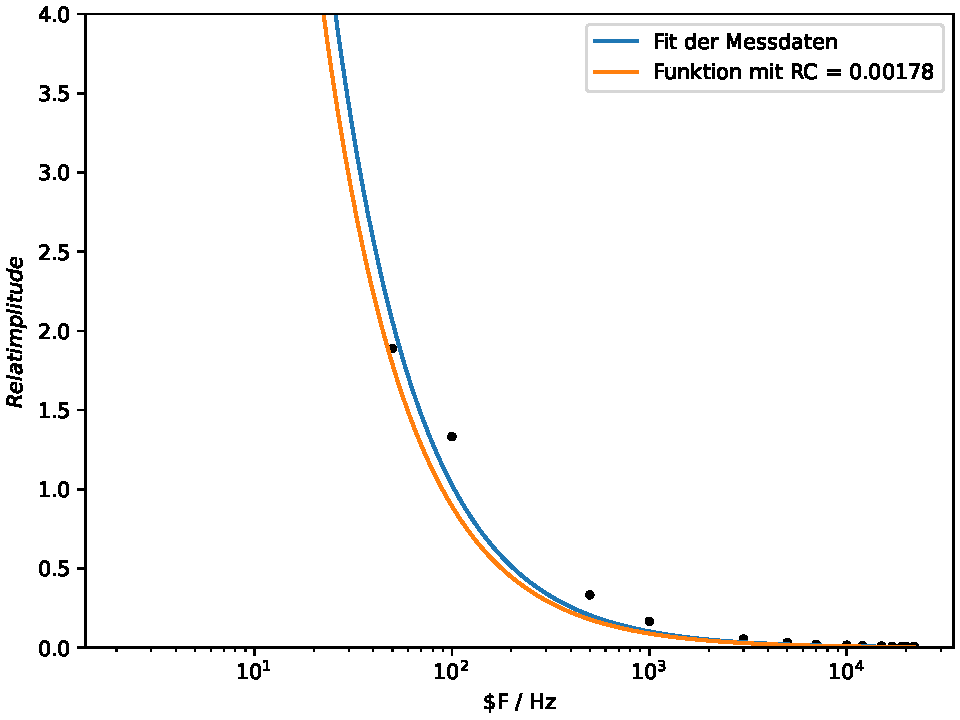
\includegraphics[width = 10cm]{plot2.pdf}
  \caption{Fit der Messwerte der Relativamplitude und Frequenz im vergleich mit Graphen mit $RC = 0.00178$}
  \label{fig:plot2}
\end{figure}

\newpage





Für eine dritte Variante der Berechnung von RC wird der Phasenunterschied zwischen der Generatorspannung und der Kondensatorspannung abhängig von der Frequenz gemessen.
Die Messeregebnisses finden sich in Tabelle \ref{tab:tabelle3}.

\begin{table}
  \centering
  \caption{Messwerte zur Phasenverschiebung und Frequenz}
  \label{tab:tabelle3}
  \sisetup{table-format=1.1, per-mode=reciprocal}
  \begin{tblr}{
      colspec = {S[table-format=3.3] S[table-format=3.3] S[table-format=5.5]},
      row{1} = {guard, mode=math},
      vline{2} = {2}{-}{text=\clap{$\pm$}},
    }
    \toprule
    \SetCell[c=2]{c} \varphi \mathbin{/} rad & & F \mathbin{/} \unit{\hertz} [\pm 1] & \\
    \midrule
    3.77  &  0.15  &  50   \\
    2.2   &  0.13  &  100  \\
    1.6   &  0.6   &  500  \\
    1.3   &  0.6   &  1000 \\
    1.9   &  0.8   &  3000 \\
    1.9   &  0.6   &  5000 \\
    1.5   &  0.4   &  7000 \\
    1,9   &  0.6   &  10000\\
    1.5   &  0.8   &  12000\\
    1.9   &  0.9   &  15000\\
    1.7   &  0.4   &  17000\\
    1.4   &  0.5   &  19000\\
    1.5   &  0.5   &  20000\\
    1.38  &  0.28  &  22000\\
    \bottomrule
  \end{tblr}
\end{table}

\newpage

Im folgenden Plot \ref{fig:plot3} werden die Messergebnisse dargestellt, zum vergleich sind auch die Kurven der eigentlich erwarteten $\arctan$ Funktion \ref{eqn:phase1} mit den beiden vorher errechneten RC werten abgebildet.


\begin{figure}
  \centering
  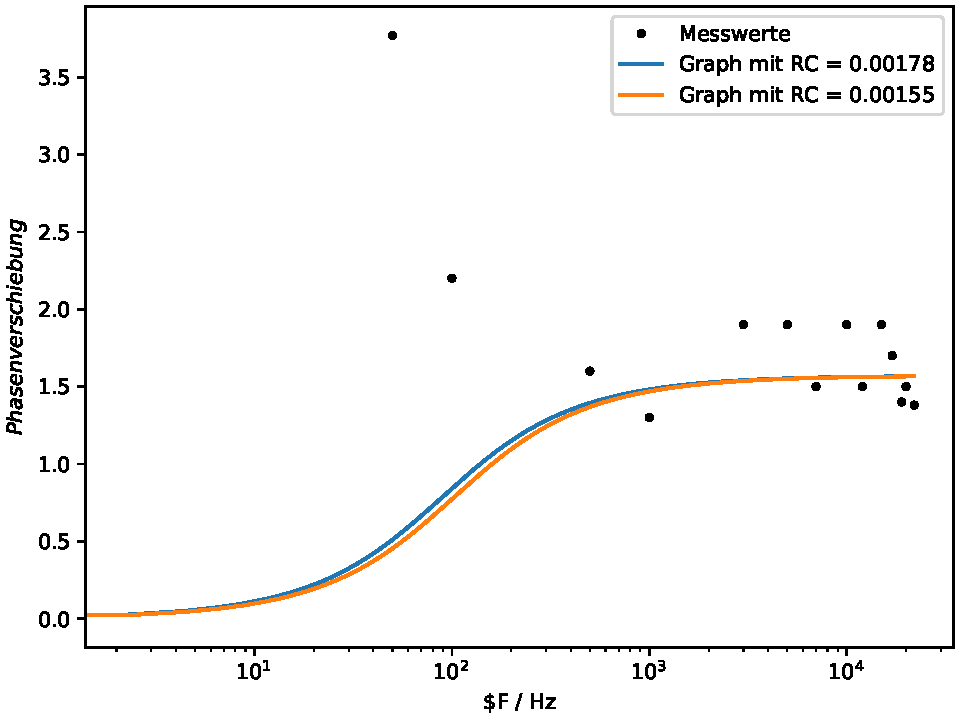
\includegraphics[width = 10cm]{plot3.pdf}
  \caption{Messwerte im Vergleich mit erwarteter Funktion}
  \label{fig:plot3}
\end{figure}

\newpage

Nun werden die Messwerte für die relative Amplitude $A_{(\omega)}/U_0$ abhängig von der Phase dargestellt in einem Polarplot.
Zum Vergleich wird ausserdem die eigentliche Funktion geplottet, die die gestalt $A/U_0 = \frac{\sin(\varphi)}{\tan(\varphi)}$ hat.

\begin{figure}
\centering
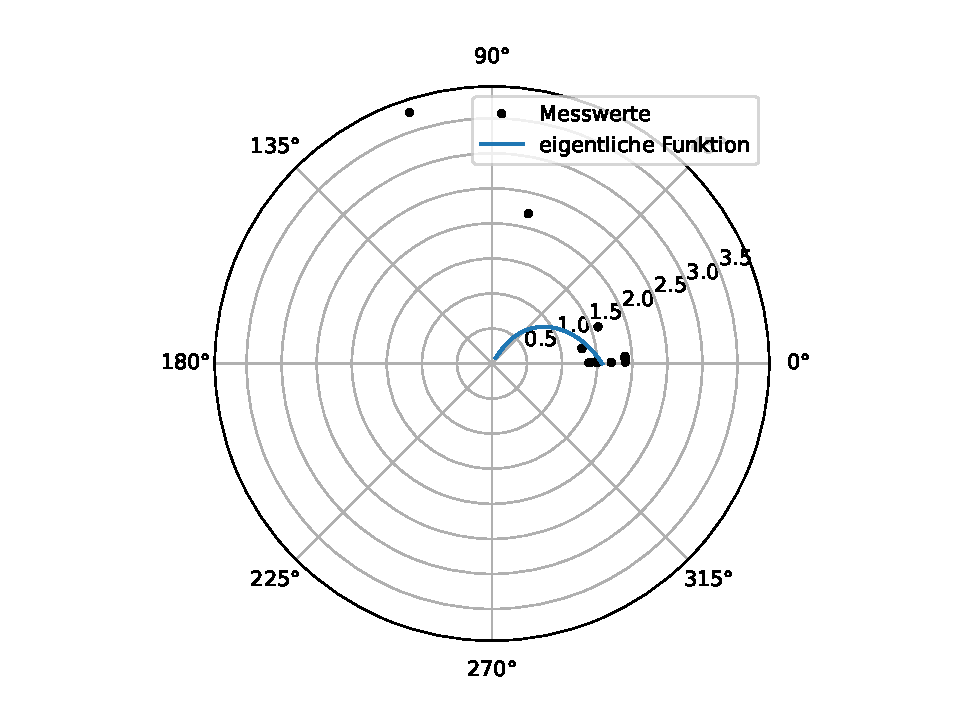
\includegraphics[width = 10cm]{plot4.pdf}
\caption{Polarplot der relativen Amplitude abhängig von der Phasenverschiebung}
\label{fig:plot4}
\end{figure}

\newpage

Zur Verifikation der Integratorfunktion werden nun 3 Abbildungen \ref{fig:int1},  \ref{fig:int2} und \ref{fig:int3} gezeigt, die jeweils eine generierte Spannung gemeinsam mit der vom Tiefpass integrierten Spannung abbilden.

\begin{figure}
  \centering
  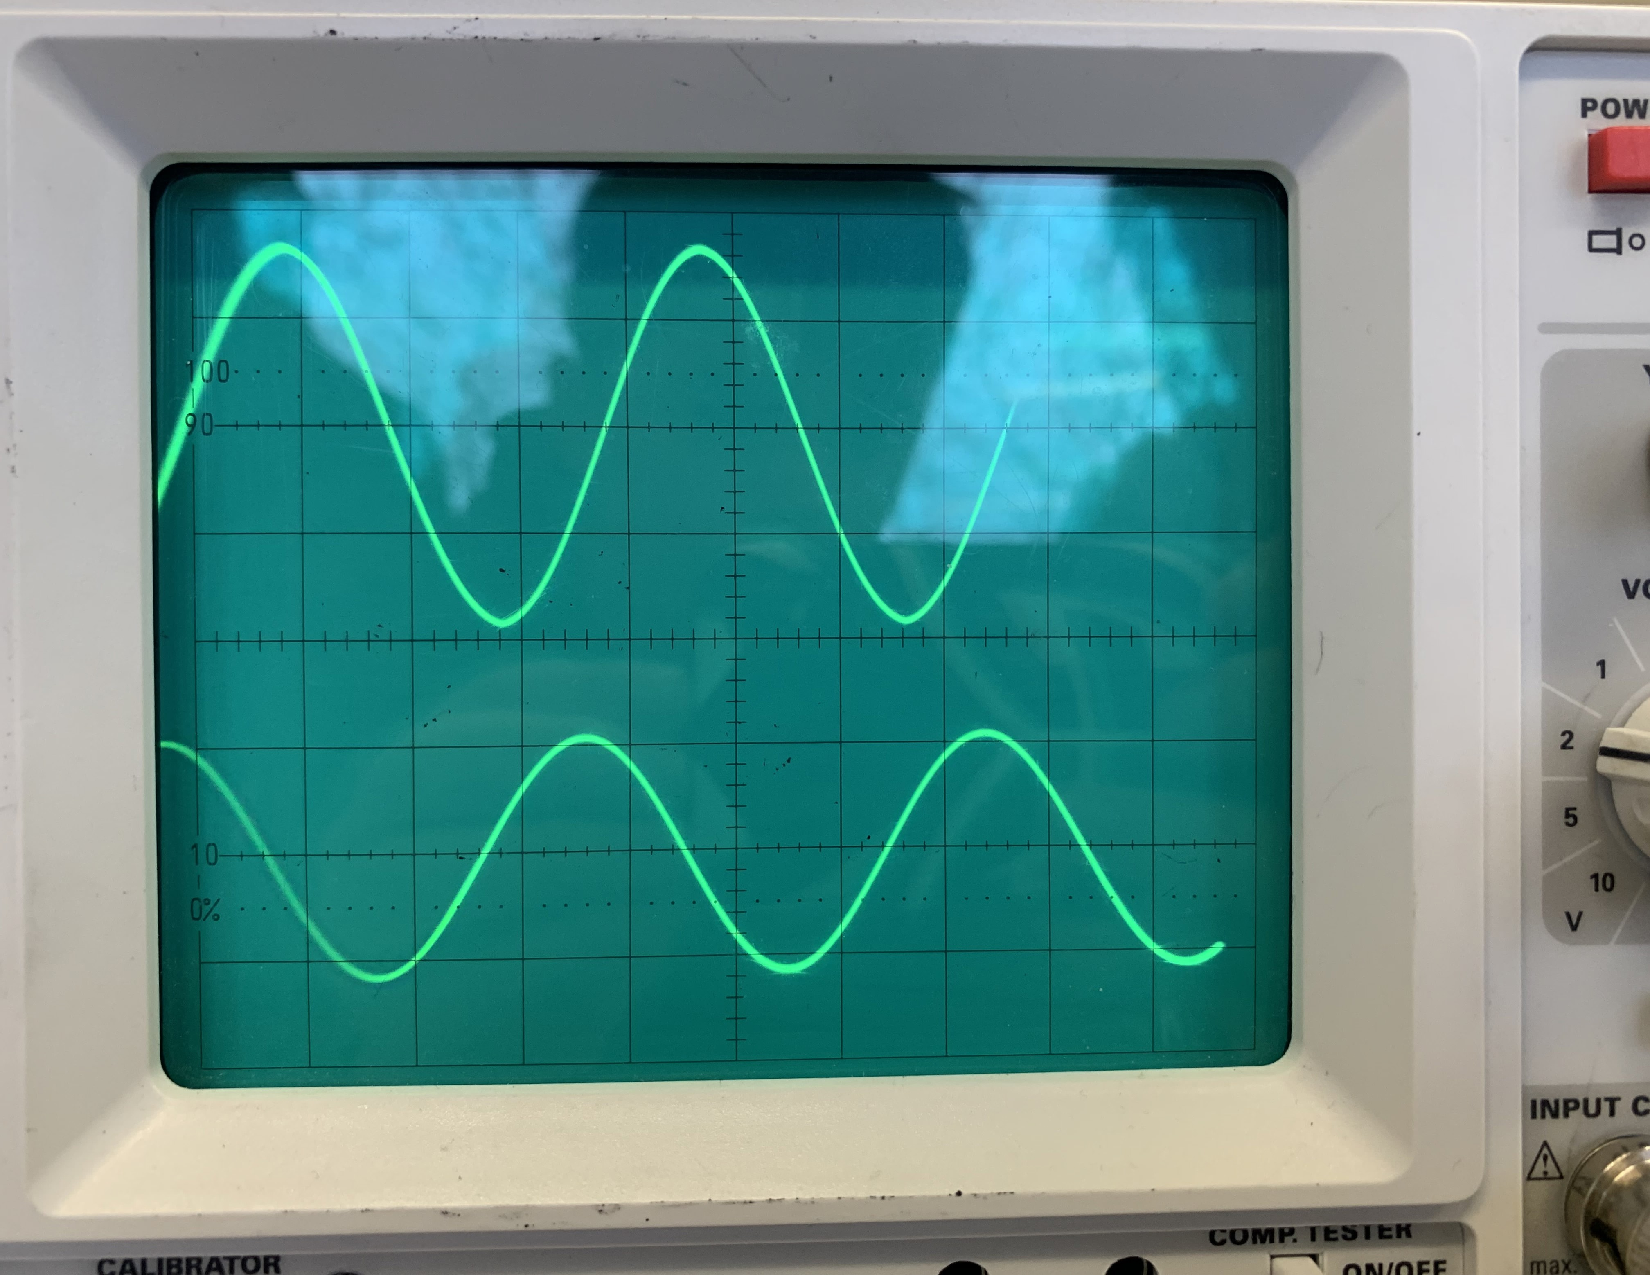
\includegraphics[width = 10cm]{V353foto1.pdf}
  \caption{Sinusspannung Integriert}
  \label{fig:int1}
\end{figure}
\begin{figure}
  \centering
  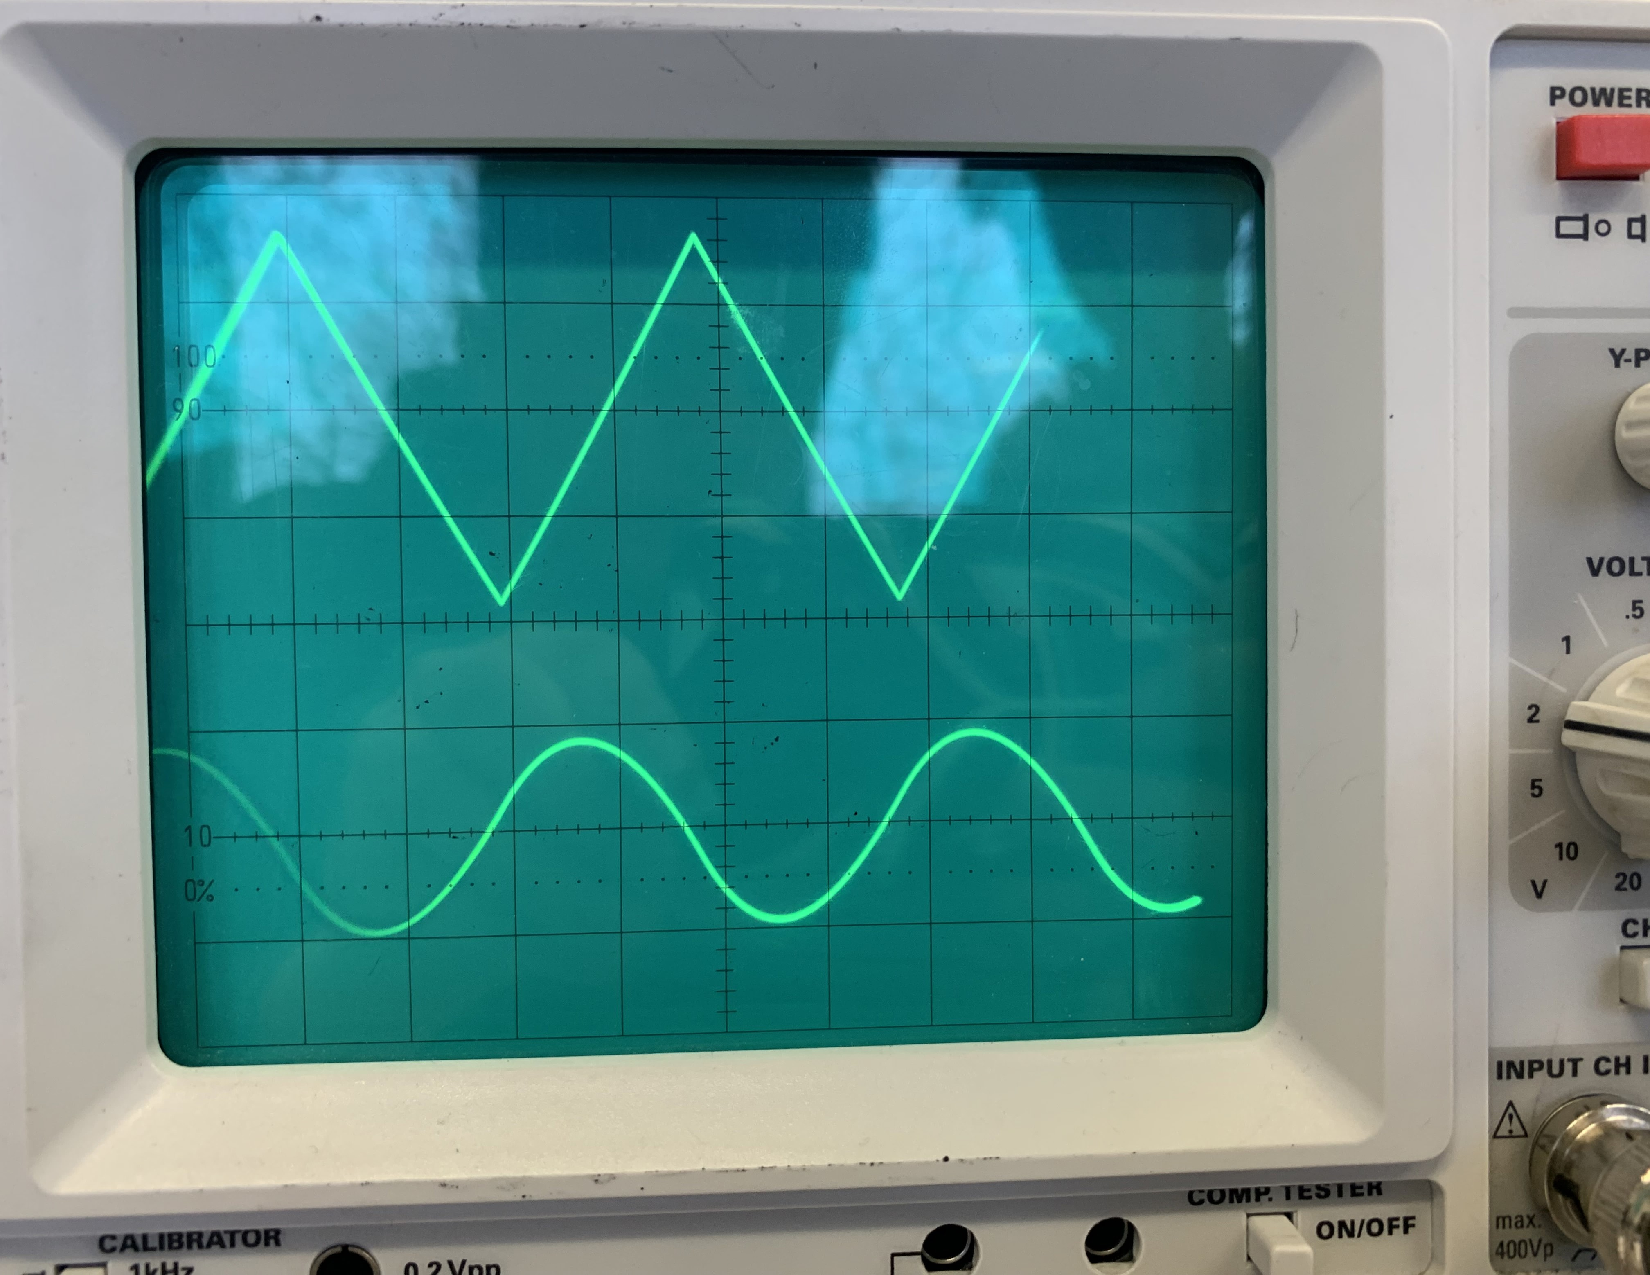
\includegraphics[width = 10cm]{V353foto2.pdf}
  \caption{Dreiecksspannung Integriert}
  \label{fig:int2}
\end{figure}
\begin{figure}
  \centering
  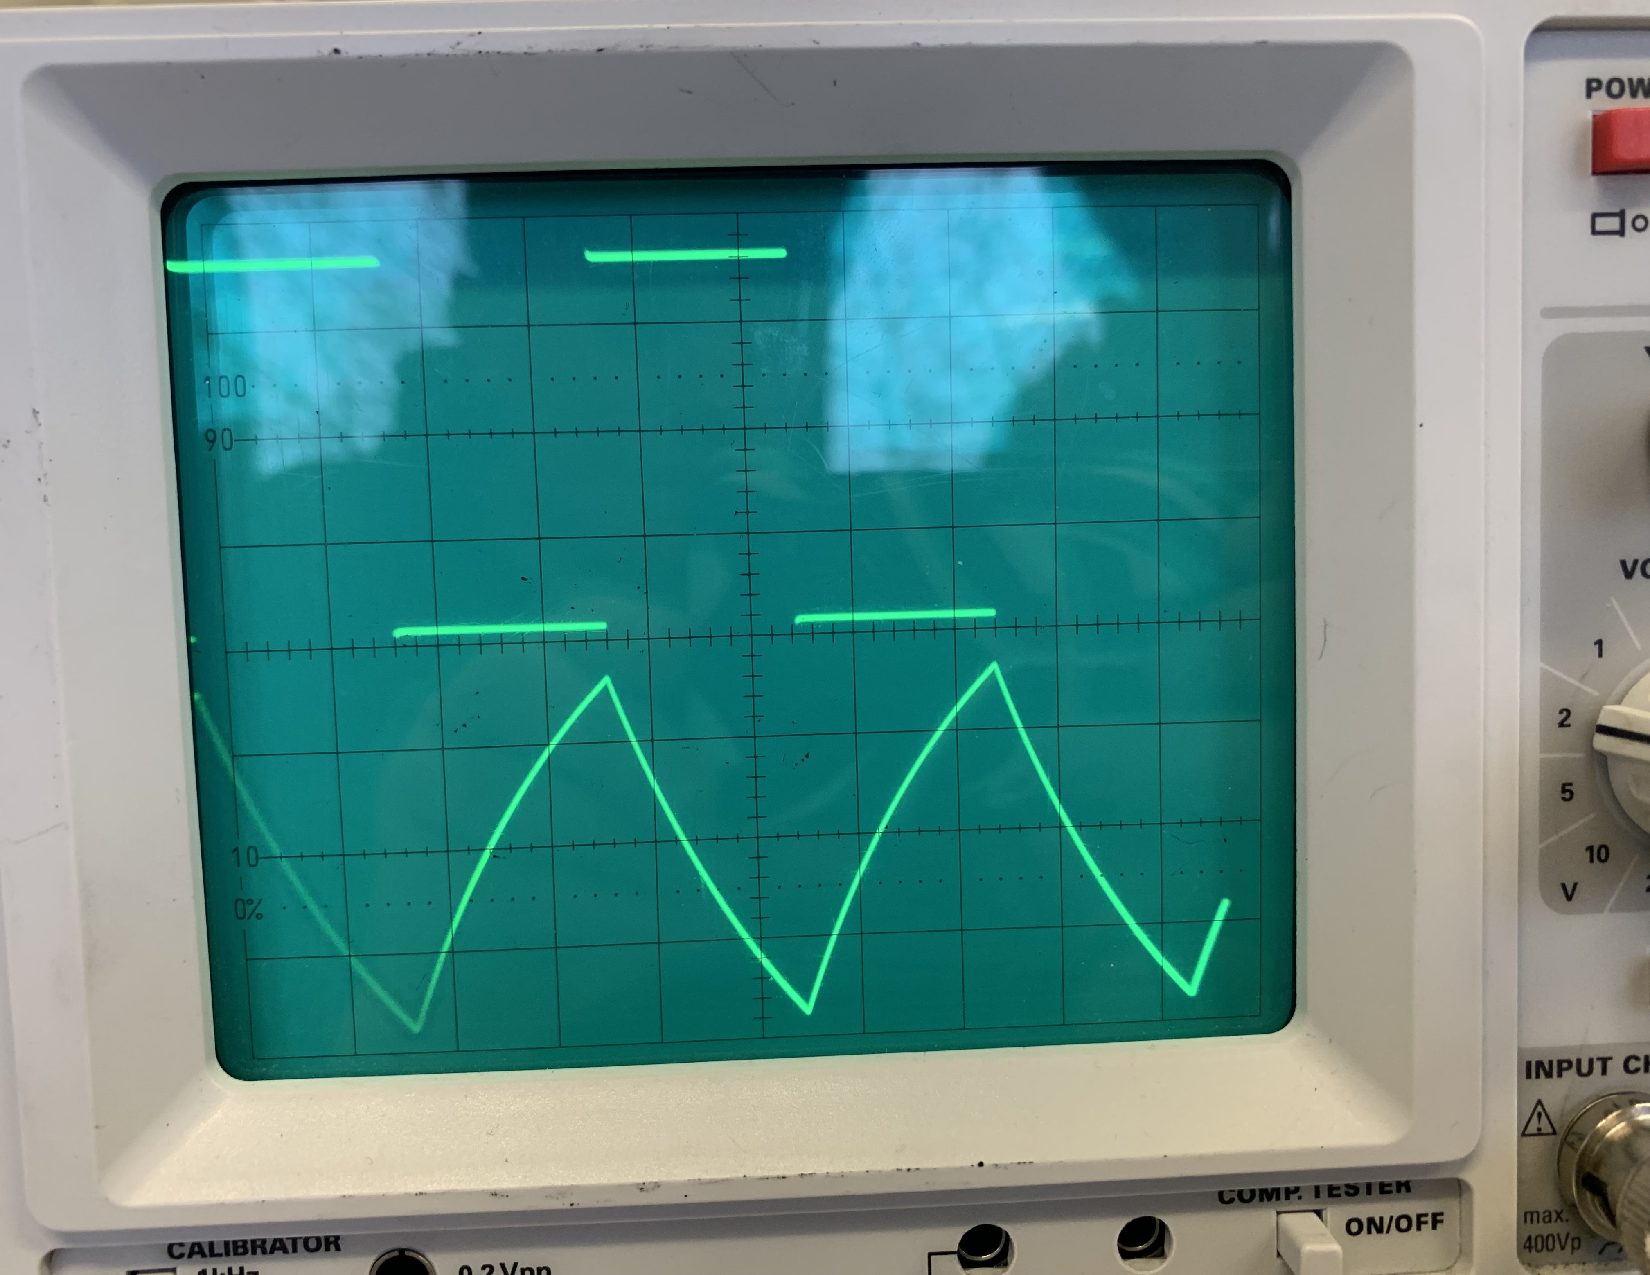
\includegraphics[width = 10cm]{V353foto3.pdf}
  \caption{Rechtecksspannung Integriert}
  \label{fig:int3}
\end{figure}









